\documentclass[12pt,a4paper,oneside]{report}

% ---------------------------------------------------------------------------
% Edit these fields before submission.
% ---------------------------------------------------------------------------
\newcommand{\ProjectTitle}{Neural Rover}
\newcommand{\ProjectSubtitle}{A Wi-Fi Controlled Mobile Monitoring Platform with Live Video and Pan--Tilt Camera}
\newcommand{\StudentName}{Student Name}
\newcommand{\StudentID}{Student ID}
\newcommand{\SupervisorName}{Supervisor Name}
\newcommand{\DepartmentName}{Department of Computer Science and Engineering}
\newcommand{\UniversityName}{University Name}
\newcommand{\CourseCode}{CSE499 Final Project}
\newcommand{\SubmissionDate}{July 2026}

\usepackage[utf8]{inputenc}
\usepackage[T1]{fontenc}
\usepackage{lmodern}
\usepackage{geometry}
\geometry{margin=1in}
\usepackage{graphicx}
\usepackage{xcolor}
\usepackage{booktabs}
\usepackage{longtable}
\usepackage{tabularx}
\usepackage{array}
\usepackage{multirow}
\usepackage{enumitem}
\usepackage{listings}
\usepackage{caption}
\usepackage{subcaption}
\usepackage{float}
\usepackage{pdflscape}
\usepackage{microtype}
\usepackage{fancyhdr}
\usepackage{titlesec}
\usepackage{hyperref}
\usepackage{url}
\usepackage{cleveref}

\definecolor{RoverBlue}{HTML}{1473E6}
\definecolor{RoverGreen}{HTML}{16A36A}
\definecolor{RoverNavy}{HTML}{0B1728}
\definecolor{RoverRed}{HTML}{C92333}
\definecolor{CodeBg}{HTML}{F4F6F8}

\hypersetup{
  colorlinks=true,
  linkcolor=RoverBlue,
  citecolor=RoverGreen,
  urlcolor=RoverBlue,
  pdftitle={\ProjectTitle: \ProjectSubtitle},
  pdfauthor={\StudentName}
}

\pagestyle{fancy}
\fancyhf{}
\fancyhead[L]{\ProjectTitle}
\fancyhead[R]{\CourseCode}
\fancyfoot[C]{\thepage}
\renewcommand{\headrulewidth}{0.4pt}

\titleformat{\chapter}[display]
  {\normalfont\bfseries\color{RoverNavy}}
  {\filleft\Large\chaptertitlename\ \thechapter}
  {1ex}
  {\titlerule\vspace{1ex}\Huge}

\setlist[itemize]{topsep=4pt,itemsep=3pt,parsep=0pt}
\setlist[enumerate]{topsep=4pt,itemsep=3pt,parsep=0pt}
\renewcommand{\arraystretch}{1.22}

\lstdefinestyle{cppstyle}{
  language=C++,
  backgroundcolor=\color{CodeBg},
  basicstyle=\ttfamily\small,
  keywordstyle=\color{RoverBlue}\bfseries,
  commentstyle=\color{RoverGreen},
  stringstyle=\color{RoverRed},
  numbers=left,
  numberstyle=\tiny\color{gray},
  stepnumber=1,
  numbersep=8pt,
  frame=single,
  rulecolor=\color{gray!35},
  breaklines=true,
  showstringspaces=false,
  tabsize=2,
  captionpos=b
}

\newcolumntype{Y}{>{\raggedright\arraybackslash}X}
\newcommand{\code}[1]{\texttt{#1}}
\newcommand{\pass}{\textcolor{RoverGreen}{\textbf{Passed}}}
\newcommand{\pending}{\textcolor{RoverRed}{\textbf{Pending}}}

\begin{document}

% ---------------------------------------------------------------------------
% Front matter
% ---------------------------------------------------------------------------
\begin{titlepage}
  \centering
  \vspace*{1.2cm}
  {\Large\bfseries \UniversityName\par}
  \vspace{0.4cm}
  {\large \DepartmentName\par}
  \vspace{1.7cm}
  {\color{RoverBlue}\rule{\textwidth}{2pt}\par}
  \vspace{0.8cm}
  {\Huge\bfseries\color{RoverNavy}\ProjectTitle\par}
  \vspace{0.45cm}
  {\LARGE\ProjectSubtitle\par}
  \vspace{0.8cm}
  {\color{RoverBlue}\rule{\textwidth}{2pt}\par}
  \vspace{1.5cm}
  {\Large\CourseCode\par}
  \vfill
  \begin{tabular}{rl}
    \textbf{Submitted by:} & \StudentName \\
    \textbf{Student ID:} & \StudentID \\
    \textbf{Supervised by:} & \SupervisorName \\
    \textbf{Submission date:} & \SubmissionDate
  \end{tabular}
  \vfill
  {\large A report submitted in partial fulfillment of the requirements of the final project course.\par}
\end{titlepage}

\pagenumbering{roman}

\chapter*{Declaration}
\addcontentsline{toc}{chapter}{Declaration}
I declare that this report describes the design and implementation of the
\ProjectTitle\ project. External technical information, datasheets, software
documentation, and research papers used in the report are acknowledged in the
references. The editable source code and diagrams associated with the prototype
are maintained with the project files.

\vspace{2cm}
\noindent
\begin{tabularx}{\textwidth}{X X}
  \rule{6cm}{0.4pt} & \rule{6cm}{0.4pt} \\
  Student signature & Date
\end{tabularx}

\chapter*{Abstract}
\addcontentsline{toc}{chapter}{Abstract}
This report presents \ProjectTitle, a four-wheel Wi-Fi controlled rover designed
as a mobile foundation for remote observation and future intelligent monitoring
in elderly-care environments. The implemented prototype combines a 30-pin ESP32
main controller, an ESP32-CAM camera module, two L298N dual H-bridge motor-driver
boards, four geared DC motors, an LM2596 step-down converter, and a two-axis
pan--tilt mechanism. A phone creates a 2.4\,GHz hotspot and opens a responsive
web interface served by the main ESP32. The interface supports press-and-hold
movement, automatic stopping after command loss, live camera viewing, pan and
tilt commands, and camera-light control.

The system separates motor power from the regulated 5\,V logic rail while
maintaining a common ground. The main ESP32 uses PWM for four motor channels,
servo pulses for pan and tilt, WebSocket communication for responsive browser
control, and UART2 to discover the camera's dynamically assigned IP address.
The ESP32-CAM supplies an MJPEG stream on port 81. During integration, the
installed sensor was found not to support hardware JPEG. The firmware was
therefore extended with an RGB565 QVGA capture path and software JPEG
conversion, allowing the stream to operate without replacing the camera.

Bench testing verified Wi-Fi connection, browser control, motor actuation,
camera streaming, and UART camera-address announcements. Final end-to-end
verification of the pan--tilt user controls remains a defined test item. The
report also proposes a second-stage laptop pipeline using face recognition,
pose estimation, event logging, and caregiver alerts. These AI functions are
future work and are intentionally separated from the completed embedded
prototype.

\tableofcontents
\listoffigures
\listoftables
\clearpage

\chapter*{Abbreviations}
\addcontentsline{toc}{chapter}{Abbreviations}
\begin{tabularx}{\textwidth}{lY}
  \toprule
  \textbf{Term} & \textbf{Meaning} \\
  \midrule
  AP & Wireless access point \\
  CAM & Camera module \\
  GPIO & General-purpose input/output \\
  H-bridge & Bidirectional DC motor-driving circuit \\
  HTTP & Hypertext Transfer Protocol \\
  MJPEG & Motion JPEG video stream \\
  PWM & Pulse-width modulation \\
  QVGA & Quarter VGA, 320$\times$240 pixels \\
  UART & Universal asynchronous receiver/transmitter \\
  VGA & Video Graphics Array, 640$\times$480 pixels \\
  \bottomrule
\end{tabularx}

\clearpage
\pagenumbering{arabic}

% ---------------------------------------------------------------------------
\chapter{Introduction}
\label{ch:introduction}

\section{Background}
Remote observation systems usually depend on fixed cameras. A fixed camera can
cover only the area visible from its mounting position, while a mobile platform
can move toward a location of interest and adjust its viewing direction.
Low-cost ESP32 hardware makes it possible to combine Wi-Fi networking, PWM,
UART communication, and a browser-based user interface on a compact embedded
platform. The ESP32 family provides the processing, communication, GPIO, UART,
and LED PWM peripherals needed for this type of prototype
\cite{esp32datasheet}.

\ProjectTitle\ applies these capabilities to a four-wheel rover. The immediate
goal is not to replace a caregiver or to act as a certified medical device.
Instead, it provides a controllable mobile camera that can later supply video to
a laptop-based perception system.

\section{Problem Statement}
The engineering problem is to integrate four DC motors, two motor drivers, a
camera stream, two servo channels, a phone-based control interface, and two
ESP32 boards without making the system unstable or difficult to operate.
Several practical constraints must be addressed:

\begin{itemize}
  \item DC motors generate electrical noise and large startup-current transients.
  \item The camera and main controller receive dynamic IP addresses from a phone
        hotspot.
  \item Browser control must remain responsive without leaving the motors active
        after communication is lost.
  \item The ESP32-CAM has limited memory and processing capacity.
  \item Camera modules sold with ESP32-CAM boards may use sensors with different
        output capabilities.
  \item The final design must preserve GPIO13 for pan and GPIO4 for tilt while
        using the remaining GPIOs for two L298N boards.
\end{itemize}

\section{Project Objectives}
The project objectives are:

\begin{enumerate}
  \item Build a four-wheel rover controlled from a phone browser.
  \item Stream live video from an ESP32-CAM over the same local network.
  \item Provide pan and tilt control for the camera mount.
  \item Drive two L298N modules with PWM-based enable signals.
  \item Use a stable power architecture based on a battery and LM2596 converter.
  \item Automatically associate the camera stream with the main control page.
  \item Implement fail-safe stopping when browser commands or Wi-Fi are lost.
  \item Prepare an expansion path for laptop-based face recognition, pose
        estimation, event logging, and caregiver alerts.
\end{enumerate}

\section{Scope and Current Status}
The report distinguishes implemented functionality from proposed functionality.
The embedded rover, local control interface, motor-control firmware, camera
server, and camera-address UART protocol have been implemented. Camera streaming
is operational using the non-JPEG fallback described in
\cref{sec:camera-fallback}. Pan--tilt GPIO allocation and firmware commands are
implemented; final user-interface verification with the installed servos is
listed as a remaining acceptance test. Face recognition, fall detection,
Telegram alerts, database storage, and chatbot queries are proposed for the
next project stage.

\section{Main Contributions}
The main contributions of the project are:

\begin{itemize}
  \item a complete two-controller rover architecture;
  \item an exact GPIO map for two L298N drivers and four motors;
  \item a responsive WebSocket-based browser controller;
  \item automatic ESP32-CAM IP discovery over UART;
  \item a split motor/logic power design with common grounding;
  \item a sensor-compatible camera fallback that converts RGB565 frames to
        browser-ready JPEG; and
  \item a documented path from embedded hardware to laptop-based AI services.
\end{itemize}

% ---------------------------------------------------------------------------
\chapter{System Requirements and Architecture}
\label{ch:architecture}

\section{Functional Requirements}
\begin{table}[H]
  \centering
  \caption{Functional requirements}
  \label{tab:functional-requirements}
  \begin{tabularx}{\textwidth}{p{1.5cm}Yp{2.4cm}}
    \toprule
    \textbf{ID} & \textbf{Requirement} & \textbf{Current state} \\
    \midrule
    FR-01 & Join the 2.4\,GHz phone hotspot named \code{CAR}. & Implemented \\
    FR-02 & Serve a phone-compatible rover control page. & Implemented \\
    FR-03 & Move forward, backward, left, right, and stop. & Implemented \\
    FR-04 & Stop automatically after command loss or Wi-Fi loss. & Implemented \\
    FR-05 & Stream live camera frames in a web browser. & Implemented \\
    FR-06 & Discover the camera IP without manually changing the main page. & Implemented \\
    FR-07 & Adjust pan, tilt, and camera light from the control page. & Firmware implemented; final servo UI test pending \\
    FR-08 & Perform face recognition and fall detection on a laptop. & Future work \\
    \bottomrule
  \end{tabularx}
\end{table}

\section{Non-Functional Requirements}
\begin{itemize}
  \item \textbf{Responsiveness:} held movement commands must be repeated while a
        direction button remains pressed.
  \item \textbf{Safety:} the rover must stop after a communication timeout.
  \item \textbf{Stability:} the ESP32 logic supply must not depend on motor-driver
        regulator behavior.
  \item \textbf{Maintainability:} pin definitions, network settings, and hardware
        roles must be explicit in the source code.
  \item \textbf{Local operation:} basic control and streaming must work without
        Internet access.
  \item \textbf{Extensibility:} the stream must be accessible to a laptop for
        future inference.
\end{itemize}

\section{System Architecture}
The phone hotspot forms the local network. The main ESP32 serves the combined
control page and controls motors and servos. The ESP32-CAM independently
provides its camera page, light-control endpoint, and MJPEG stream. The camera
periodically transmits a \code{CAMIP:<address>} line to the main ESP32 through
UART. Once the main controller parses the address, the browser embeds
\code{http://<camera-ip>:81/stream}.

\begin{landscape}
\begin{figure}[p]
  \centering
  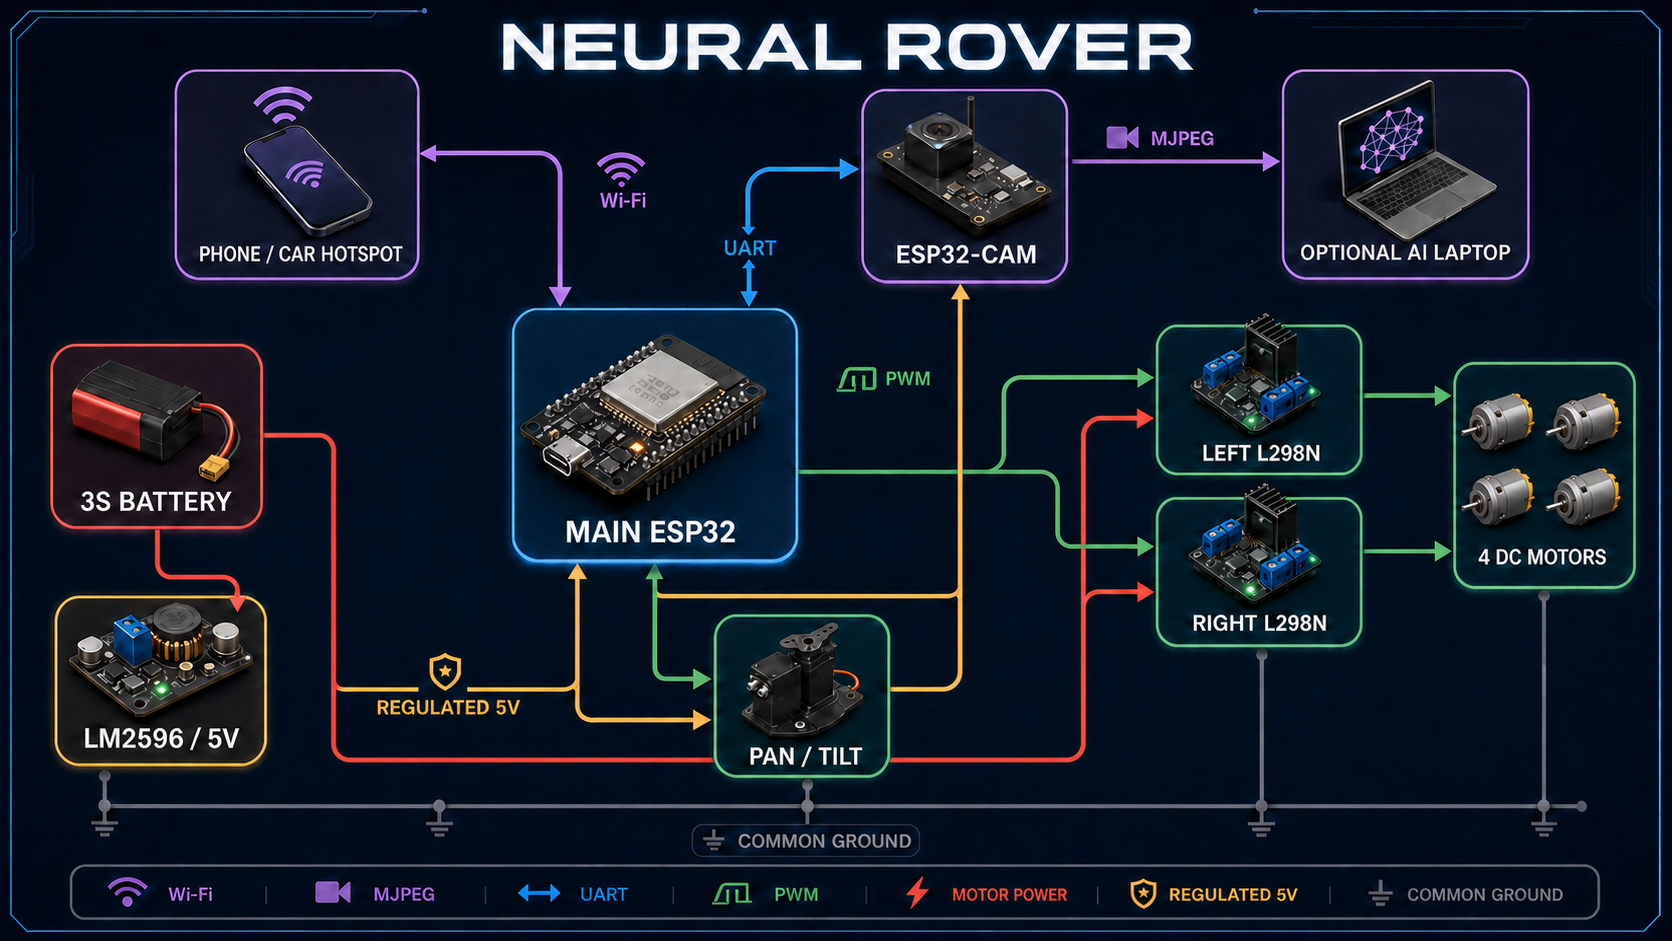
\includegraphics[width=0.95\linewidth]{assets/architecture.png}
  \caption{Complete Neural Rover architecture, signal map, and power
  distribution.}
  \label{fig:architecture}
\end{figure}
\end{landscape}

\section{End-to-End Data Flow}
The principal data and control flow is:

\begin{enumerate}
  \item The phone enables hotspot \code{CAR} using the configured password.
  \item Both ESP32 boards join as Wi-Fi stations using the Arduino ESP32 Wi-Fi
        API \cite{esp32wifi}.
  \item The user opens the dynamic IP printed by the main ESP32.
  \item The browser opens a WebSocket to the main controller and an MJPEG stream
        to the camera.
  \item Pressing a direction button sends a one-character command and starts a
        periodic held-command heartbeat.
  \item The main ESP32 converts the command into motor directions and PWM duty.
  \item Pan and tilt slider messages carry an axis prefix and angle.
  \item The camera periodically announces its IP over UART, allowing recovery
        after hotspot reconnection or address changes.
\end{enumerate}

\section{Design Rationale}
The two-board design prevents video streaming from consuming the control
controller's resources. It also allows the camera server and motor-control loop
to restart independently. A local hotspot was selected because it requires no
router configuration and keeps control functional when Internet connectivity is
unavailable. WebSocket communication was selected for movement because it
provides a persistent bidirectional channel and avoids loading a new page for
each command.

% ---------------------------------------------------------------------------
\chapter{Hardware Design}
\label{ch:hardware}

\section{Bill of Materials}
\begin{longtable}{p{0.8cm}p{4.3cm}p{2.0cm}p{7.2cm}}
  \caption{Principal hardware components}
  \label{tab:bom}\\
  \toprule
  \textbf{No.} & \textbf{Component} & \textbf{Quantity} & \textbf{Role} \\
  \midrule
  \endfirsthead
  \toprule
  \textbf{No.} & \textbf{Component} & \textbf{Quantity} & \textbf{Role} \\
  \midrule
  \endhead
  1 & ESP32 development board, 30 pin & 1 & Main controller, Wi-Fi server, WebSocket handler, PWM, servos, and UART2 \\
  2 & AI-Thinker-style ESP32-CAM board & 1 & Camera capture, MJPEG stream, flash control, and camera-IP announcement \\
  3 & L298N dual H-bridge module & 2 & Bidirectional control of left and right motor pairs \\
  4 & Geared DC motor & 4 & Front-left, rear-left, front-right, and rear-right propulsion \\
  5 & SG90-class servo & 2 & Pan and tilt movement \\
  6 & LM2596 adjustable buck converter & 1 & Regulated 5\,V rail \\
  7 & 3S rechargeable battery & 1 & Primary energy source \\
  8 & Four-wheel rover chassis and wheels & 1 set & Mechanical structure \\
  9 & Jumper wires, terminal wiring, and connectors & As required & Signal, power, and grounding connections \\
  10 & Phone with 2.4\,GHz hotspot and browser & 1 & Local network and user interface \\
  \bottomrule
\end{longtable}

The L298 is a dual full-bridge driver intended for bidirectional inductive loads
such as DC motors \cite{l298}. Two modules are used so that left and right
motor pairs have independent direction and PWM-enable paths.

\section{Power Architecture}
The battery supplies the motor voltage directly to the two L298N motor-power
inputs and also feeds the LM2596 input. The LM2596 is a step-down switching
regulator family suitable for producing a lower DC rail from a higher input
\cite{lm2596}. The converter is adjusted to 5.0\,V before connection to logic.

\begin{equation}
  V_{\text{logic}} = 5.0~\text{V}
\end{equation}

The regulated rail supplies:

\begin{itemize}
  \item the main ESP32 through its 5\,V/VIN input;
  \item the ESP32-CAM through its 5\,V input;
  \item both servo VCC connections; and
  \item the L298N logic rail when the module is configured for external 5\,V.
\end{itemize}

All grounds are tied together. This common reference is required for GPIO,
PWM, UART, and servo pulses to be interpreted correctly. The ENA and ENB jumper
caps are removed because the main ESP32 actively drives those pins with PWM.
If external 5\,V is applied to an L298N logic input, the module's onboard
5V-enable jumper must be configured according to that specific board to avoid
connecting two regulator outputs together.

\section{Main ESP32 Pin Assignment}
\begin{table}[H]
  \centering
  \caption{Main controller GPIO allocation}
  \label{tab:main-gpio}
  \begin{tabularx}{\textwidth}{YcYc}
    \toprule
    \textbf{Left-side function} & \textbf{GPIO} &
    \textbf{Right-side function} & \textbf{GPIO} \\
    \midrule
    Left ENA (front PWM) & 25 & Right ENA (front PWM) & 32 \\
    Left IN1 & 26 & Right IN1 & 23 \\
    Left IN2 & 27 & Right IN2 & 22 \\
    Left IN3 & 14 & Right IN3 & 21 \\
    Left IN4 & 12 & Right IN4 & 19 \\
    Left ENB (rear PWM) & 33 & Right ENB (rear PWM) & 18 \\
    \midrule
    Pan servo signal & 13 & Tilt servo signal & 4 \\
    Camera UART RX2 & 16 & Camera UART TX2 & 17 \\
    \bottomrule
  \end{tabularx}
\end{table}

\section{Motor Output Assignment}
\begin{table}[H]
  \centering
  \caption{Motor-to-driver output assignment}
  \label{tab:motor-output}
  \begin{tabularx}{\textwidth}{YYY}
    \toprule
    \textbf{Driver} & \textbf{Output terminals} & \textbf{Motor position} \\
    \midrule
    Left L298N & OUT1--OUT2 & Front-left motor \\
    Left L298N & OUT3--OUT4 & Rear-left motor \\
    Right L298N & OUT1--OUT2 & Front-right motor \\
    Right L298N & OUT3--OUT4 & Rear-right motor \\
    \bottomrule
  \end{tabularx}
\end{table}

Motor polarity determines which electrical state produces physical forward
rotation. During commissioning, each wheel is lifted from the surface and
tested individually. If a wheel rotates opposite to the required direction,
its two output wires are swapped rather than changing the entire control map.

\section{Servo Interface}
The main ESP32 generates a 50\,Hz servo signal. An angle in the range
$0^\circ$--$180^\circ$ is mapped to an approximate pulse width of
0.5--2.5\,ms:

\begin{equation}
  t_{\text{pulse}} =
  500~\mu\text{s} +
  \frac{\theta}{180^\circ}\left(2000~\mu\text{s}\right).
\end{equation}

The pan signal is connected to GPIO13 and the tilt signal to GPIO4. Servo power
is taken from the regulated 5\,V rail rather than the ESP32 3.3\,V pin.

\section{UART Wiring}
UART wires are crossed because a transmitter must connect to a receiver:

\begin{center}
\begin{tabular}{rcl}
  ESP32-CAM U0T/TX & $\longrightarrow$ & Main ESP32 GPIO16/RX2 \\
  ESP32-CAM U0R/RX & $\longleftarrow$ & Main ESP32 GPIO17/TX2 \\
  ESP32-CAM GND & $\longleftrightarrow$ & Main ESP32 GND
\end{tabular}
\end{center}

The configured baud rate is 115200 bit/s using 8 data bits, no parity, and one
stop bit.

% ---------------------------------------------------------------------------
\chapter{Firmware and Web Software}
\label{ch:software}

\section{Software Organization}
Two Arduino sketches implement the system:

\begin{itemize}
  \item \code{ESP32\_Controller.ino}: main Wi-Fi connection, WebSocket server,
        HTML interface, motors, servo PWM, fail-safe logic, and camera UART.
  \item \code{ESP32\_CAM\_Controller.ino}: camera initialization, stream server,
        light endpoint, Wi-Fi reconnection, mDNS, and camera-IP announcement.
\end{itemize}

\section{Main Controller Initialization}
During \code{setup()}, the main controller:

\begin{enumerate}
  \item starts the USB serial port at 115200 bit/s;
  \item configures motor direction pins and PWM enable outputs;
  \item configures the two servo outputs;
  \item starts UART2 on GPIO16 and GPIO17;
  \item connects to hotspot \code{CAR};
  \item registers the WebSocket and HTTP routes; and
  \item starts the asynchronous web server on port 80.
\end{enumerate}

Wi-Fi persistence is disabled to reduce unnecessary flash writes, Wi-Fi sleep
is disabled for control responsiveness, and automatic reconnection is enabled.

\section{Motor State Machine}
The motion command is represented by an enumeration containing stop, forward,
backward, left, and right states. A direction change first disables motor PWM
and waits for a short dead time. PWM then ramps upward instead of applying the
maximum duty instantly. This reduces mechanical shock and the instantaneous
current demand of four motors.

\begin{lstlisting}[style=cppstyle,caption={Simplified command-to-motion interface}]
enum Motion : uint8_t {
  STOP = 0,
  FORWARD = 1,
  BACKWARD = 2,
  LEFT = 3,
  RIGHT = 4
};

void requestMotion(Motion nextMotion) {
  requestedMotion = nextMotion;
  lastCommandMs = millis();
}
\end{lstlisting}

\section{Fail-Safe Behavior}
The browser repeats a held command periodically. The main controller records
the time of the most recent valid command. If no valid command is received
within the configured timeout, it requests \code{STOP}. Wi-Fi loss also requests
an immediate stop. This means a disconnected phone or closed browser does not
leave the rover intentionally driving.

\section{Web Interface}
The HTML, CSS, and JavaScript interface is stored in program memory and served
from the main ESP32. The layout is optimized for phone use and includes:

\begin{itemize}
  \item a camera-stream panel and camera connection indicator;
  \item forward, backward, left, right, and stop buttons;
  \item a displayed current-motion state;
  \item pan and tilt sliders from $0^\circ$ to $180^\circ$; and
  \item a camera-light slider from 0 to 255.
\end{itemize}

\begin{figure}[H]
  \centering
  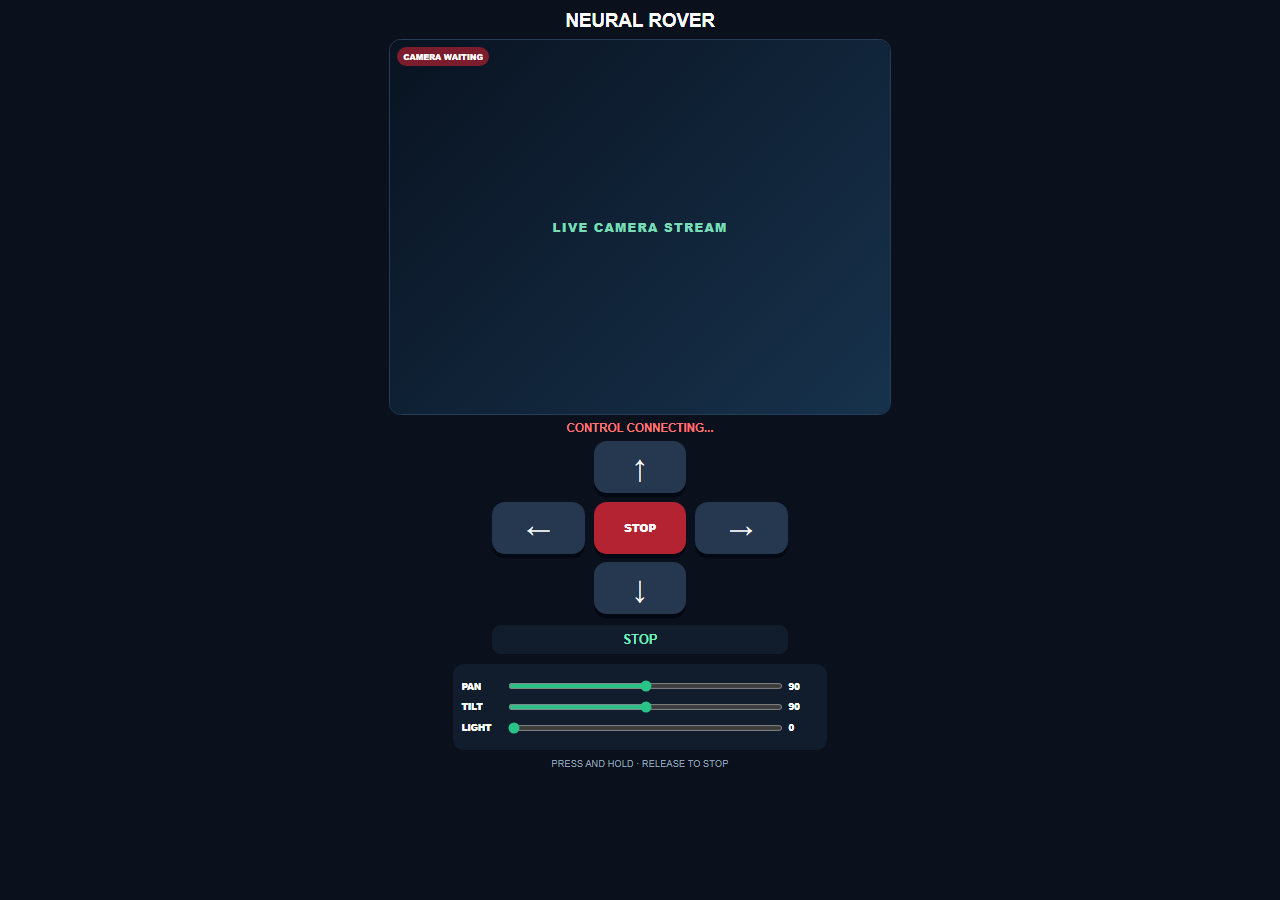
\includegraphics[width=0.86\textwidth]{assets/controller-ui.png}
  \caption{Responsive Neural Rover web interface generated from the current
  controller firmware.}
  \label{fig:controller-ui}
\end{figure}

Pointer-down events start movement and pointer-up, pointer-cancel, page-hide,
window-blur, and visibility-change events request stop. This event coverage is
important on mobile browsers where a finger may leave the button area or the
page may be backgrounded.

\section{Camera IP Discovery}
The camera periodically prints:

\begin{center}
\code{CAMIP:192.168.x.x}
\end{center}

The main ESP32 reads UART2 one line at a time. A line beginning with
\code{CAMIP:} is validated as an IP address and stored. The browser polls the
main controller's \code{/camera-ip} route and updates the image source when the
address changes. The main board also sends \code{?} periodically so the camera
can respond immediately.

\section{Camera HTTP Services}
The camera sketch runs two HTTP servers:

\begin{table}[H]
  \centering
  \caption{ESP32-CAM HTTP endpoints}
  \label{tab:camera-endpoints}
  \begin{tabularx}{\textwidth}{p{3.3cm}p{2cm}Y}
    \toprule
    \textbf{Endpoint} & \textbf{Port} & \textbf{Purpose} \\
    \midrule
    \code{/} & 80 & Camera diagnostic page \\
    \code{/flash?value=n} & 80 & Set camera-light PWM from 0 to 255 \\
    \code{/stream} & 81 & Multipart MJPEG stream \\
    \bottomrule
  \end{tabularx}
\end{table}

\section{Non-JPEG Sensor Fallback}
\label{sec:camera-fallback}
The initial VGA/JPEG configuration returned error 0x106 and reported that JPEG
format was not supported by the installed sensor. The Espressif camera driver
supports multiple sensors, but not every supported sensor produces compressed
JPEG. Its documentation also recommends QVGA or lower for non-JPEG capture on
the original ESP32 because RGB or YUV frame transfers place greater load on
memory and Wi-Fi \cite{esp32camera}.

The camera firmware therefore performs two initialization attempts:

\begin{enumerate}
  \item request hardware JPEG at VGA for a JPEG-capable sensor;
  \item if the driver returns \code{ESP\_ERR\_NOT\_SUPPORTED}, retry using
        RGB565 at QVGA with one frame buffer.
\end{enumerate}

When a captured frame is not already JPEG, \code{frame2jpg()} converts it before
the HTTP server sends the multipart chunk. This solution provides a working
320$\times$240 stream with the installed sensor. Replacing the camera with a
genuine OV2640 would allow the hardware-JPEG VGA path.

% ---------------------------------------------------------------------------
\chapter{Implementation and Validation}
\label{ch:validation}

\section{Development Environment}
The firmware was developed and uploaded using Arduino IDE with the Espressif
Arduino core. The main controller uses the \code{ESP32 Dev Module} board
selection. The camera uses \code{AI Thinker ESP32-CAM}. Serial monitoring is
performed at 115200 baud.

\section{Main ESP32 Upload Procedure}
\begin{enumerate}
  \item Disconnect or isolate motor power during firmware upload.
  \item Connect the ESP32 development board by a data-capable USB cable.
  \item Select the CP2102 COM port rather than the computer's fixed COM1 port.
  \item Upload \code{ESP32\_Controller.ino}.
  \item Open Serial Monitor at 115200 baud and press EN.
  \item Confirm that the board prints its hotspot connection and dynamic URL.
\end{enumerate}

The first upload issue was caused by the missing Silicon Labs CP2102 virtual COM
driver. Installing the driver allowed the development board to appear as a new
COM port.

\section{ESP32-CAM Upload Procedure}
The ESP32-CAM has no onboard USB programmer. An Arduino Uno can be used as a USB
serial bridge with the Uno microcontroller held in reset:

\begin{center}
\begin{tabular}{rcl}
  ESP32-CAM U0T & $\rightarrow$ & Uno RX/0 \\
  ESP32-CAM U0R & $\leftarrow$ & Uno TX/1 through 3.3\,V level conversion \\
  ESP32-CAM GND & $\leftrightarrow$ & Uno GND \\
  ESP32-CAM 5V & $\leftarrow$ & Stable 5\,V supply \\
  ESP32-CAM GPIO0 & $\rightarrow$ & GND during upload only \\
  Uno RESET & $\rightarrow$ & Uno GND
\end{tabular}
\end{center}

GPIO0 must be disconnected from ground after upload. A reset with GPIO0 still
low produces \code{DOWNLOAD\_BOOT} and \code{waiting for download}; with GPIO0
released, normal flash boot is reported.

\section{Test Method}
Testing was performed incrementally to avoid confusing software, wiring, and
power faults:

\begin{enumerate}
  \item upload and serial-test each board separately;
  \item verify the hotspot sees two clients;
  \item test the camera diagnostic page and direct stream;
  \item lift the rover so all wheels can rotate without moving the chassis;
  \item test each motor-driver channel;
  \item test the main controller page without motor load;
  \item apply motor power and repeat direction commands;
  \item connect UART and confirm camera-IP discovery;
  \item test loss-of-command stopping; and
  \item test pan, tilt, and light controls.
\end{enumerate}

\section{Verification Results}
\begin{table}[H]
  \centering
  \caption{Current verification status}
  \label{tab:test-results}
  \begin{tabularx}{\textwidth}{p{0.9cm}Yp{2.4cm}}
    \toprule
    \textbf{ID} & \textbf{Test} & \textbf{Result} \\
    \midrule
    T-01 & Main ESP32 joins hotspot \code{CAR} and receives an IP address. & \pass \\
    T-02 & Main web page loads from a phone on the same hotspot. & \pass \\
    T-03 & Forward, backward, left, right, and stop commands reach the firmware. & \pass \\
    T-04 & All four motors can be actuated through the two L298N boards. & \pass \\
    T-05 & ESP32-CAM joins the hotspot and serves its diagnostic page. & \pass \\
    T-06 & Direct camera stream opens on port 81. & \pass \\
    T-07 & Camera transmits repeating \code{CAMIP} announcements over UART. & \pass \\
    T-08 & Main page receives the camera address and embeds the stream. & \pass \\
    T-09 & Main firmware contains pan/tilt commands on GPIO13/GPIO4. & \pass \\
    T-10 & Installed pan/tilt mechanism verified from the final page controls. & \pending \\
    T-11 & Laptop face recognition and fall detection. & Future phase \\
    \bottomrule
  \end{tabularx}
\end{table}

\section{Engineering Problems and Resolutions}
\begin{longtable}{p{3.6cm}p{5.0cm}p{6.4cm}}
  \caption{Problems encountered during integration}
  \label{tab:problems}\\
  \toprule
  \textbf{Observed behavior} & \textbf{Diagnosis} & \textbf{Resolution} \\
  \midrule
  \endfirsthead
  \toprule
  \textbf{Observed behavior} & \textbf{Diagnosis} & \textbf{Resolution} \\
  \midrule
  \endhead
  Only COM1 appeared & CP2102 driver was absent & Installed the Silicon Labs
  virtual COM driver and selected the newly detected port. \\
  Upload reported no serial data & ESP32-CAM was not in download mode or UART
  TX/RX was reversed & Crossed U0T/U0R correctly, grounded GPIO0, and manually
  reset when the uploader began connecting. \\
  Camera remained in \code{waiting for download} & GPIO0 was still grounded
  after upload & Removed GPIO0 from GND and reset the board. \\
  Commands initially worked and then stalled under motor power & Battery charge,
  voltage sag, ground routing, and motor noise affected the controller & Used
  direct battery motor power, regulated 5\,V logic power, a common ground, and
  incremental driver testing. \\
  Camera section remained on ``connecting'' & The main ESP32 had not learned the
  camera's IP & Corrected UART wiring and added periodic \code{CAMIP}
  announcements and requests. \\
  Camera initialization failed with 0x106 & Installed sensor did not support
  hardware JPEG & Added the RGB565 QVGA fallback and software JPEG conversion. \\
  \bottomrule
\end{longtable}

\section{Discussion}
The integration history shows that apparent network or firmware failures may be
caused by power delivery and wiring. Serial logs were essential for separating
reset events, download mode, Wi-Fi connection, camera initialization, and UART
activity. The final design is more robust because it incorporates explicit
timeouts, reconnect behavior, camera-address announcements, PWM ramping, and a
sensor-compatible video path.

% ---------------------------------------------------------------------------
\chapter{Proposed Intelligent Monitoring Extension}
\label{ch:ai}

\section{Laptop-Based Processing}
The ESP32-CAM is used as a network camera rather than an inference platform.
A GPU-capable laptop connected to hotspot \code{CAR} can read:

\begin{center}
\code{http://<camera-ip>:81/stream}
\end{center}

Moving the AI workload to a laptop avoids the memory and compute limitations of
the original ESP32 while preserving the low-cost camera and control hardware.

\section{Face Detection and Recognition}
The proposed pipeline first detects and aligns a face, generates a feature
embedding, and compares the embedding with enrolled residents. ArcFace uses an
additive angular margin to learn discriminative face embeddings
\cite{arcface}. A practical pipeline would include:

\begin{enumerate}
  \item collect consented enrollment images;
  \item detect and align faces;
  \item generate normalized embeddings;
  \item store embeddings under a resident identifier;
  \item compare live embeddings using a validated threshold; and
  \item log a recognition only when image quality and confidence requirements
        are met.
\end{enumerate}

The current QVGA stream is sufficient for testing detection at short distances,
but recognition performance is expected to fall when a face occupies few
pixels, is more than approximately 1.5\,m away, or is viewed at a large yaw
angle. A genuine OV2640 or higher-quality camera, improved lighting, a raised
mount, and deliberate camera positioning would improve the usable input.

\section{Pose and Fall Detection}
BlazePose is a real-time body-pose model designed to track body landmarks from
video \cite{blazepose}. MediaPipe provides a framework for composing perception
pipelines \cite{mediapipe}. The proposed rover would classify temporal pose
sequences rather than treating a single horizontal body detection as a fall.
Useful signals include:

\begin{itemize}
  \item rapid vertical displacement of the torso;
  \item a transition from standing to lying;
  \item low hip and shoulder positions relative to the frame;
  \item persistence of a lying posture; and
  \item absence of recovery movement for a configured duration.
\end{itemize}

Alerts should be treated as decision support. A caregiver should review the
image or stream before acting when conditions permit.

\section{Event Log and Caregiver Interface}
Each detection event may contain:

\begin{itemize}
  \item timestamp;
  \item resident identifier or ``unknown'';
  \item rover zone;
  \item detection confidence;
  \item posture state;
  \item image reference; and
  \item alert acknowledgement state.
\end{itemize}

A Telegram bot or web dashboard could answer questions such as ``Who has not
been seen in the last two hours?'' or ``Show today's fall events.'' An LLM
should query structured, permission-controlled data rather than inventing
answers from an unconstrained conversation.

\section{Proposed Work Plan}
\begin{figure}[H]
  \centering
  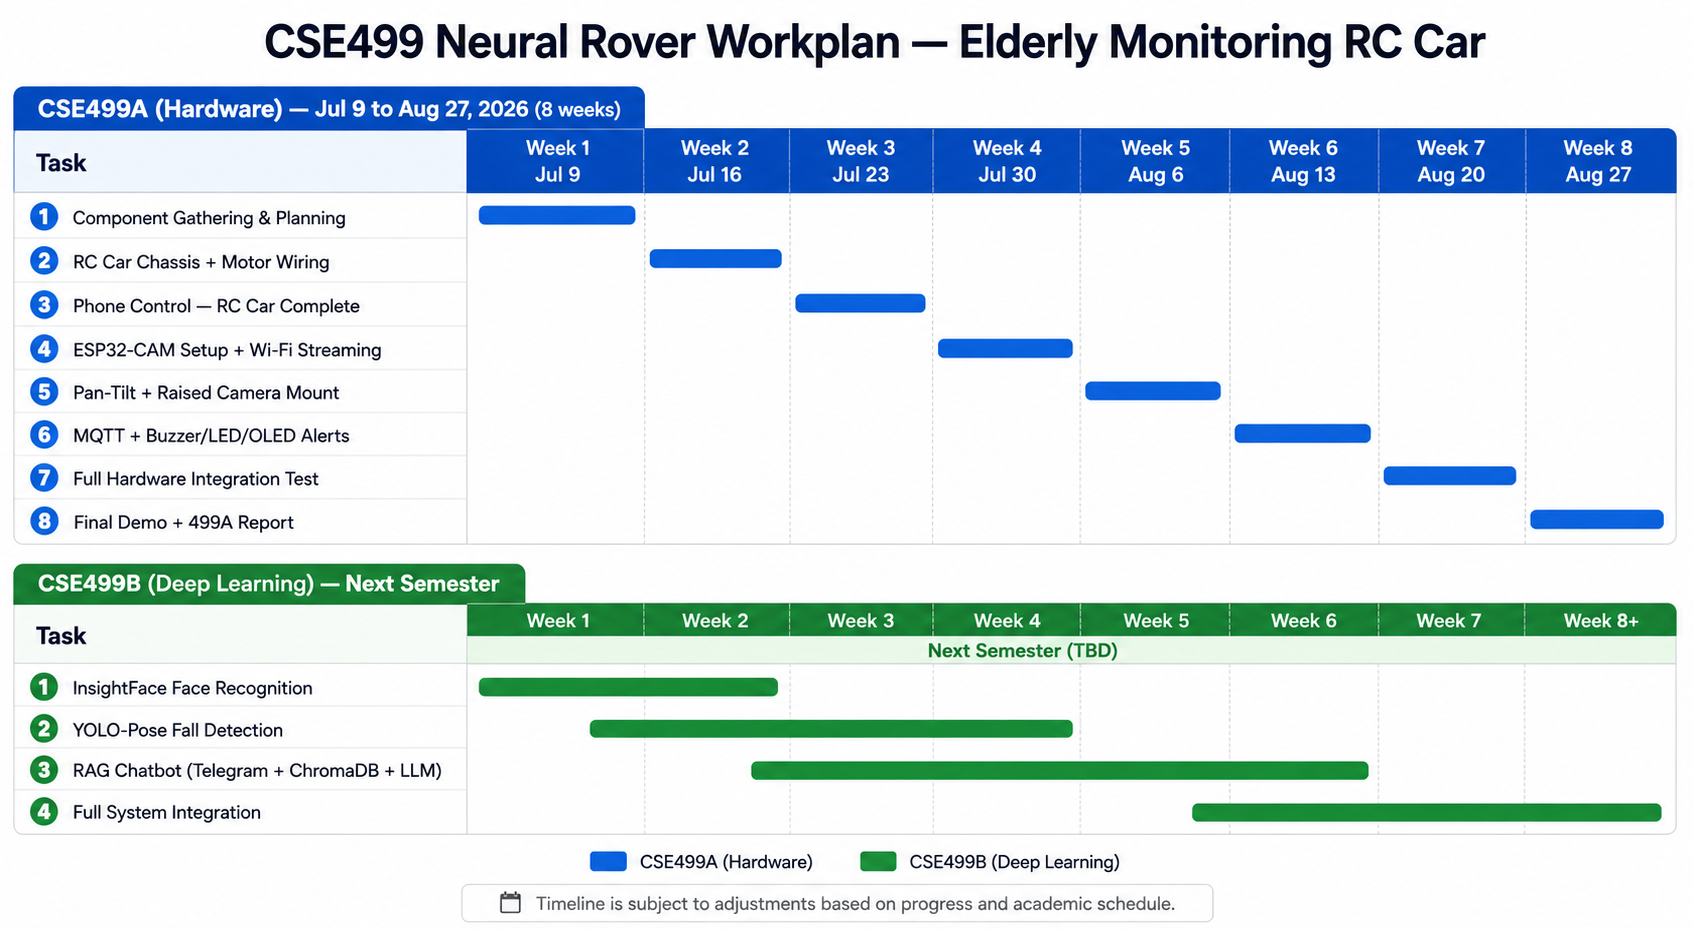
\includegraphics[width=\textwidth]{assets/workplan.png}
  \caption{Hardware and deep-learning development work plan.}
  \label{fig:workplan}
\end{figure}

% ---------------------------------------------------------------------------
\chapter{Limitations, Safety, and Ethics}
\label{ch:limitations}

\section{Current Technical Limitations}
\begin{itemize}
  \item The present fallback stream is QVGA rather than VGA.
  \item Camera frame rate is limited by software JPEG conversion.
  \item Hotspot-assigned IP addresses may change after reconnection.
  \item L298N drivers have a significant voltage drop compared with modern
        MOSFET motor drivers.
  \item The platform has no wheel encoders, so motion is open-loop.
  \item The prototype does not yet measure battery voltage.
  \item Pan--tilt end-to-end acceptance testing remains incomplete.
  \item The rover does not perform autonomous obstacle avoidance.
\end{itemize}

\section{Electrical and Mechanical Safety}
Testing should begin with the wheels raised. Wiring must be changed only when
power is off. The buck converter output must be measured before connection.
Motor stalls should be avoided because stall current may exceed the safe
continuous capability of wiring, batteries, or driver modules. The battery
requires an appropriate charger and protection method. Servos should have
mechanical travel limits that prevent cable strain.

\section{Privacy and Responsible Use}
Video and biometric processing in an elderly-care environment require informed
consent, access control, data minimization, retention limits, and a clear human
review process. Face recognition can produce false matches, and pose detection
can produce false alarms or missed events. The system must therefore not be
described as a medical device or as a substitute for professional supervision.
Raw video and face embeddings should be encrypted at rest where stored, and
only authorized caregivers should access the stream or event log.

\section{Threat Model}
The current prototype uses a shared hotspot password and unencrypted HTTP. For
deployment beyond a controlled demonstration, the following improvements are
required:

\begin{itemize}
  \item change default credentials and avoid embedding production secrets in
        source code;
  \item authenticate the control page;
  \item isolate the rover network from untrusted clients;
  \item protect remote access with a secure gateway or VPN;
  \item sign firmware and control update access; and
  \item log administrative and caregiver access.
\end{itemize}

% ---------------------------------------------------------------------------
\chapter{Conclusion and Future Work}
\label{ch:conclusion}

\section{Conclusion}
\ProjectTitle\ demonstrates that a low-cost two-ESP32 architecture can combine
four-motor mobility, a phone-hosted local network, browser control, live camera
streaming, servo-ready pan--tilt control, and automatic camera discovery. The
project's most important engineering outcome is not a single feature but the
integration of power, networking, embedded control, and camera streaming into a
repeatable platform.

The final firmware includes practical recovery mechanisms: Wi-Fi reconnection,
command-loss stopping, PWM ramping, direction dead time, repeated camera-IP
announcements, and a non-JPEG sensor fallback. These mechanisms directly address
problems observed during testing and make the design easier to diagnose and
extend.

\section{Recommended Next Steps}
The recommended order of future work is:

\begin{enumerate}
  \item complete the final pan--tilt UI acceptance test;
  \item replace or confirm the camera sensor if smoother VGA is required;
  \item add bulk capacitance and motor-noise suppression near the drivers;
  \item add battery-voltage monitoring and low-voltage shutdown;
  \item add wheel encoders or closed-loop speed control;
  \item add an ultrasonic or time-of-flight obstacle sensor;
  \item build a laptop stream receiver and frame-quality monitor;
  \item evaluate face detection before recognition;
  \item evaluate temporal pose/fall detection using consented test scenarios;
  \item add secure event storage and caregiver notifications; and
  \item validate privacy, reliability, and false-alarm behavior before any care
        environment trial.
\end{enumerate}

% ---------------------------------------------------------------------------
\appendix
\chapter{Quick Operating Procedure}

\section{Normal Startup}
\begin{enumerate}
  \item Confirm all wiring and common grounds with power off.
  \item Enable the 2.4\,GHz phone hotspot \code{CAR}.
  \item Apply battery power and regulated 5\,V power.
  \item Wait for both ESP32 boards to join the hotspot.
  \item Open the main ESP32 IP address printed in Serial Monitor.
  \item Confirm that the page reports control connection and camera live status.
  \item Lift the wheels for the first movement test.
  \item Press and hold a direction button; release it to stop.
\end{enumerate}

\section{Direct Camera Test}
If the embedded stream does not load:

\begin{enumerate}
  \item check that the hotspot shows two connected clients;
  \item open \code{http://<camera-ip>/};
  \item open \code{http://<camera-ip>:81/stream};
  \item check main Serial Monitor for
        \code{ESP32-CAM detected at: http://...};
  \item verify U0T$\rightarrow$GPIO16, U0R$\leftarrow$GPIO17, and common ground;
        and
  \item reset the ESP32-CAM first, then the main ESP32.
\end{enumerate}

\chapter{Camera Module Pin Map}
\begin{longtable}{p{5cm}p{3cm}p{7cm}}
  \caption{AI-Thinker-style ESP32-CAM camera pin definitions}\\
  \toprule
  \textbf{Signal} & \textbf{GPIO} & \textbf{Function} \\
  \midrule
  \endfirsthead
  \toprule
  \textbf{Signal} & \textbf{GPIO} & \textbf{Function} \\
  \midrule
  \endhead
  PWDN & 32 & Camera power-down control \\
  RESET & --1 & No dedicated reset GPIO \\
  XCLK & 0 & Camera external clock \\
  SIOD & 26 & SCCB/I\textsuperscript{2}C-like data \\
  SIOC & 27 & SCCB/I\textsuperscript{2}C-like clock \\
  Y9 & 35 & Camera data bit \\
  Y8 & 34 & Camera data bit \\
  Y7 & 39 & Camera data bit \\
  Y6 & 36 & Camera data bit \\
  Y5 & 21 & Camera data bit \\
  Y4 & 19 & Camera data bit \\
  Y3 & 18 & Camera data bit \\
  Y2 & 5 & Camera data bit \\
  VSYNC & 25 & Vertical synchronization \\
  HREF & 23 & Horizontal reference \\
  PCLK & 22 & Pixel clock \\
  Flash LED & 4 & Onboard light PWM \\
  \bottomrule
\end{longtable}

\chapter{Project Source Files}
\begin{itemize}
  \item \code{Project Car Code/ESP32\_Controller/ESP32\_Controller.ino}
  \item \code{Project Car Code/ESP32\_CAM\_Controller/ESP32\_CAM\_Controller.ino}
  \item \code{Project Files/Neural Rover Full Project Diagram.svg}
  \item \code{NEURAL\_ROVER.md}
\end{itemize}

\bibliographystyle{IEEEtran}
\bibliography{references}

\end{document}
